% ============================================================================
%  Chapitre 7, partie I : Caractériser la trajectoire
% ============================================================================

% ----------------------------------------------------------------------------
\section{Caractériser la trajectoire}
% ----------------------------------------------------------------------------

On cherche à décrire la trajectoire du centre $G$ dans le plan du sol
uniquement à partir de grandeurs exprimées dans le repère de la sphère,
c'est-à-dire celles que donnent la centrale inertielle et le filtre du
chapitre précédent : $\vect{\omega}$, $\dot{\vect{\omega}}$ et
$\vect{\gamma}$.

\begin{definition}[Vitesse et cap]
    Tant que $\vect{v}_G \neq \vect{0}$, on écrit
    \begin{equation}
        \vect{v}_G = v\,(\cos\chi\,\vect{e}_x + \sin\chi\,\vect{e}_y)
    \end{equation}
    avec $v = \|\vect{v}_G\| > 0$ la vitesse et $\chi$ le cap. Le cap satisfait :
    \begin{equation}
        \chi = \operatorname{atan2}(v_y, v_x)
    \end{equation}
\end{definition}

On note dans la suite
\begin{equation}
    \vect{u} = \vect{\omega}\wedge\vect{\gamma}
\end{equation}

\begin{proposition}[Vitesse]
    \begin{equation}
        \vect{v}_G = a\,\mat{R}\,\vect{u},
        \qquad
        v = a\,\|\vect{\omega}\wedge\vect{\gamma}\|
    \end{equation}
\end{proposition}

\begin{remarque}
    $\vect{u}\cdot\vect{\gamma} = 0$, donc $\vect{v}_G\cdot\vect{e}_z = 0$ c'est-à-dire
    le centre reste bien dans un plan horizontal. La vitesse ne s'annule que
    si $\vect{\omega}$ est colinéaire à $\vect{\gamma}$, c'est-à-dire si la
    sphère pivote sur place autour de la verticale.
\end{remarque}

\begin{proposition}[Taux de cap]
    Si $v > 0$,
    \begin{equation}
        \dot{\chi} = -\,\frac{(\vect{\omega}\wedge\vect{\gamma})\cdot\dot{\vect{\omega}}}
        {\|\vect{\omega}\wedge\vect{\gamma}\|^2}
    \end{equation}
\end{proposition}

\begin{demonstration}
    
    \textbf{Formule du cap : }
    avec $\vect{v}_G = \dot{\vect{r}} = (\dot{x}, \dot{y}, 0)$ et $\chi = \operatorname{atan2}(\dot{y}, \dot{x})$,
    \begin{equation*}
        \dot{\chi} = \frac{\dot{x}\,\ddot{y} - \dot{y}\,\ddot{x}}{\dot{x}^2 + \dot{y}^2}
        = \frac{\dot{x}\,\ddot{y} - \dot{y}\,\ddot{x}}{v^2}
    \end{equation*}
    et le numérateur est la composante verticale de $\dot{\vect{r}}\wedge\ddot{\vect{r}}$ :
    \begin{equation*}
        \dot{\chi} = \frac{\vect{e}_z\cdot(\dot{\vect{r}}\wedge\ddot{\vect{r}})}{v^2}
    \end{equation*}
    \textbf{Passage dans le repère de la sphère : }
    avec $\dot{\mat{R}} = \mat{R}\,\hatx{\vect{\omega}}$,
    \begin{equation*}
        \ddot{\vect{r}} = a\,\mat{R}\,(\dot{\vect{u}} + \vect{\omega}\wedge\vect{u})
    \end{equation*}
    donc, avec $\vect{e}_z = \mat{R}\vect{\gamma}$ et $v = a\|\vect{u}\|$,
    \begin{equation*}
        \dot{\chi} = \frac{\vect{\gamma}\cdot\big(\vect{u}\wedge(\dot{\vect{u}} + \vect{\omega}\wedge\vect{u})\big)}{\|\vect{u}\|^2}
    \end{equation*}
    \textbf{Terme de pivotement : }
    par le double produit vectoriel et $\vect{u}\cdot\vect{\omega} = 0$,
    \begin{equation*}
        \vect{u}\wedge(\vect{\omega}\wedge\vect{u})
        = \|\vect{u}\|^2\vect{\omega} - (\vect{u}\cdot\vect{\omega})\,\vect{u}
        = \|\vect{u}\|^2\vect{\omega}
    \end{equation*}
    d'où
    \begin{equation*}
        \dot{\chi} = \vect{\omega}\cdot\vect{\gamma}
        + \frac{\vect{\gamma}\cdot(\vect{u}\wedge\dot{\vect{u}})}{\|\vect{u}\|^2}
    \end{equation*}
    \textbf{Dérivée de $\vect{u}$ : }
    avec $\dot{\vect{\gamma}} = \vect{\gamma}\wedge\vect{\omega}$,
    \begin{equation*}
        \dot{\vect{u}} = \dot{\vect{\omega}}\wedge\vect{\gamma}
        + \vect{\omega}\wedge(\vect{\gamma}\wedge\vect{\omega})
    \end{equation*}
    Par le produit mixte, on a $\vect{\gamma}\cdot(\vect{u}\wedge\dot{\vect{u}}) = \dot{\vect{u}}\cdot(\vect{\gamma}\wedge\vect{u})$
    et, comme $\|\vect{\gamma}\| = 1$,
    \begin{equation*}
        \vect{\gamma}\wedge\vect{u} = \vect{\gamma}\wedge(\vect{\omega}\wedge\vect{\gamma})
        = \vect{\omega} - (\vect{\omega}\cdot\vect{\gamma})\,\vect{\gamma}
        = \vect{\omega}_\perp
    \end{equation*}
    \textbf{Premier terme : }
    \begin{equation*}
        (\dot{\vect{\omega}}\wedge\vect{\gamma})\cdot\vect{\omega}_\perp
        = (\dot{\vect{\omega}}\wedge\vect{\gamma})\cdot\big(\vect{\omega} - (\vect{\omega}\cdot\vect{\gamma})\,\vect{\gamma}\big)
        = (\dot{\vect{\omega}}\wedge\vect{\gamma})\cdot\vect{\omega}
        = \dot{\vect{\omega}}\cdot(\vect{\gamma}\wedge\vect{\omega})
        = -\,\dot{\vect{\omega}}\cdot\vect{u}
    \end{equation*}
    \textbf{Second terme : }
    $\vect{\omega}\wedge(\vect{\gamma}\wedge\vect{\omega}) = \|\vect{\omega}\|^2\vect{\gamma} - (\vect{\omega}\cdot\vect{\gamma})\,\vect{\omega}$, et
    \begin{equation*}
        \big(\|\vect{\omega}\|^2\vect{\gamma} - (\vect{\omega}\cdot\vect{\gamma})\,\vect{\omega}\big)\cdot\vect{\omega}_\perp
        = -\,(\vect{\omega}\cdot\vect{\gamma})\big(\|\vect{\omega}\|^2 - (\vect{\omega}\cdot\vect{\gamma})^2\big)
        = -\,(\vect{\omega}\cdot\vect{\gamma})\,\|\vect{u}\|^2
    \end{equation*}
    car $\vect{\gamma}\cdot\vect{\omega}_\perp = 0$ et
    $\|\vect{\omega}\wedge\vect{\gamma}\|^2 = \|\vect{\omega}\|^2 - (\vect{\omega}\cdot\vect{\gamma})^2$.

    \textbf{Conclusion : }
    \begin{equation*}
        \dot{\chi} = \vect{\omega}\cdot\vect{\gamma}
        - \frac{\dot{\vect{\omega}}\cdot\vect{u}}{\|\vect{u}\|^2}
        - \vect{\omega}\cdot\vect{\gamma}
        = -\,\frac{\vect{u}\cdot\dot{\vect{\omega}}}{\|\vect{u}\|^2}
    \end{equation*}
\end{demonstration}

\begin{exemple}[Sphère isotrope]
    Si $\mat{I} = I\,\Id$, $\vect{\Omega}$ est constant, donc
    $\dot{\vect{\omega}} = \mat{R}^T\dot{\vect{\Omega}} - \vect{\omega}\wedge\vect{\omega} = \vect{0}$.
    Alors $\dot{\chi} = 0$ et $v$ est constant : la trajectoire est une droite
    parcourue à vitesse constante. Toute courbure de la trajectoire vient donc
    de l'anisotropie de $\mat{I}$.
\end{exemple}

\begin{corollaire}[Reconstruction de la trajectoire]
    À partir de $(\vect{\omega}, \dot{\vect{\omega}}, \vect{\gamma})$ sur $[0, t]$,
    \begin{equation}
        \chi(t) = \chi_0 + \int_0^t \dot{\chi}\,\mathrm{d}s,
        \qquad
        \vect{r}(t) = \vect{r}_0 + \int_0^t v\,(\cos\chi\,\vect{e}_x + \sin\chi\,\vect{e}_y)\,\mathrm{d}s
    \end{equation}
    La trajectoire est donc connue à un déplacement près : une translation
    $\vect{r}_0$ et une rotation $\chi_0$.
\end{corollaire}

\begin{remarque} En revanche, $\chi_0$ n'est pas
    observable avec un gyromètre et un accéléromètre, rien dans
    $(\vect{\omega}, \vect{\gamma})$ ne fixe la direction du nord. Il
    faudrait un magnétomètre.
\end{remarque}

\begin{figure}[htbp]
    \centering
    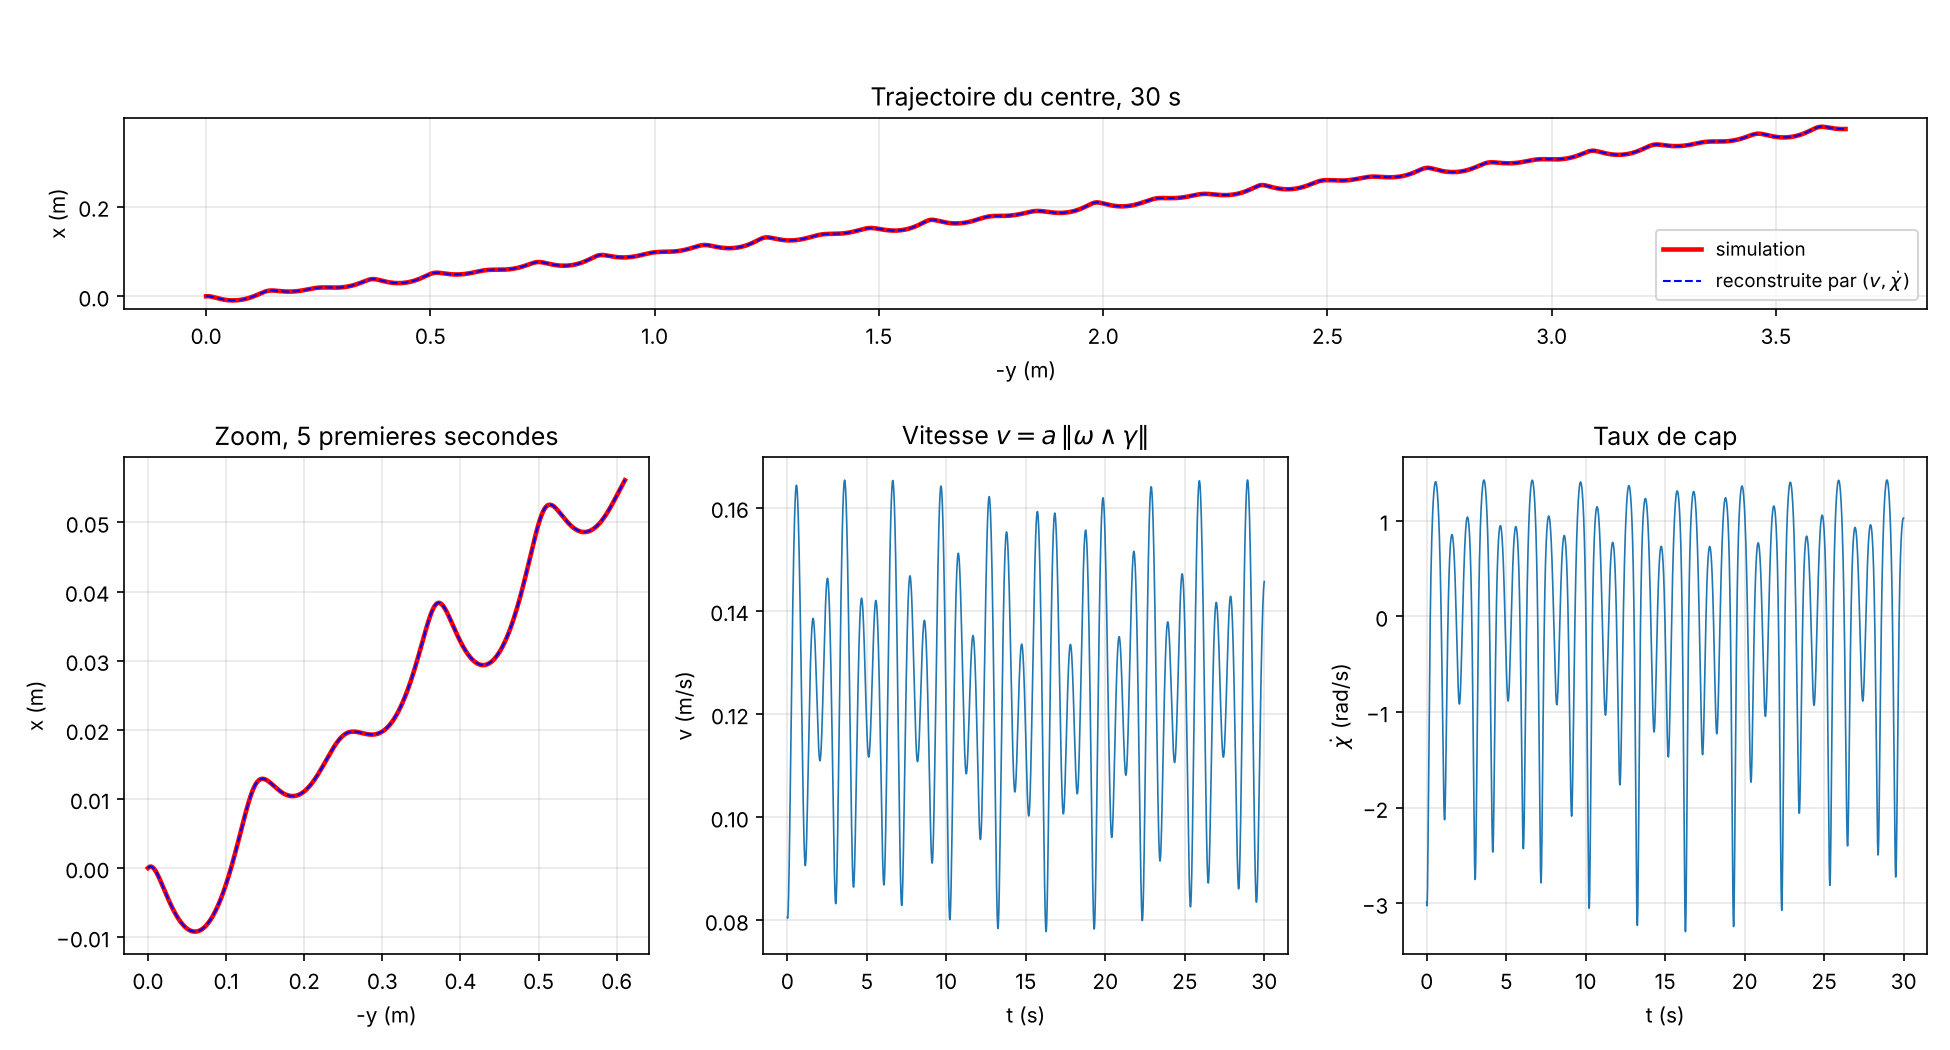
\includegraphics[width=\linewidth]{chapitre7/figures/trajectoire_intrinseque.png}
    \caption{Trajectoire simulée sur 30 s et trajectoire reconstruite par
    $(v, \dot{\chi})$.}
    \label{fig:trajectoire_intrinseque}
\end{figure}
